%%%%%%%%%%%%%%%%%%%%%%%%%%%%%%%%%%%%%%%%%
% Masters/Doctoral Thesis 
% LaTeX Template
% Version 1.41 (9/9/13)
%
% This template has been downloaded from:
% http://www.latextemplates.com
%
% Original authors:
% Steven Gunn 
% http://users.ecs.soton.ac.uk/srg/softwaretools/document/templates/
% and
% Sunil Patel
% http://www.sunilpatel.co.uk/thesis-template/
%
% License:
% CC BY-NC-SA 3.0 (http://creativecommons.org/licenses/by-nc-sa/3.0/)
%
% Note:
% Make sure to edit document variables in the Thesis.cls file
%
%%%%%%%%%%%%%%%%%%%%%%%%%%%%%%%%%%%%%%%%%

%----------------------------------------------------------------------------------------
%	PACKAGES AND OTHER DOCUMENT CONFIGURATIONS
%----------------------------------------------------------------------------------------

\documentclass[11pt, a4paper, oneside]{Thesis} % Paper size, default font size and one-sided paper

\graphicspath{{Pictures/}} % Specifies the directory where pictures are stored

\usepackage[square, numbers, comma, sort&compress]{natbib} % Use the natbib reference package - read up on this to edit the reference style; if you want text (e.g. Smith et al., 2012) for the in-text references (instead of numbers), remove 'numbers' 
\hypersetup{urlcolor=blue, colorlinks=true} % Colors hyperlinks in blue - change to black if annoying
\title{\ttitle} % Defines the thesis title - don't touch this

\begin{document}

\frontmatter % Use roman page numbering style (i, ii, iii, iv...) for the pre-content pages

\setstretch{1.3} % Line spacing of 1.3

% Define the page headers using the FancyHdr package and set up for one-sided printing
\fancyhead{} % Clears all page headers and footers
\rhead{\thepage} % Sets the right side header to show the page number
\lhead{} % Clears the left side page header

\pagestyle{fancy} % Finally, use the "fancy" page style to implement the FancyHdr headers

\newcommand{\HRule}{\rule{\linewidth}{0.5mm}} % New command to make the lines in the title page

% PDF meta-data
\hypersetup{pdftitle={\ttitle}}
\hypersetup{pdfsubject=\subjectname}
\hypersetup{pdfauthor=\authornames}
\hypersetup{pdfkeywords=\keywordnames}

%----------------------------------------------------------------------------------------
%	TITLE PAGE
%----------------------------------------------------------------------------------------

\begin{titlepage}
\begin{center}

\textsc{\LARGE \univname}\\[1.5cm] % University name
\textsc{\Large Master's Thesis}\\[0.5cm] % Thesis type

\HRule \\[0.4cm] % Horizontal line
{\huge \bfseries \ttitle}\\[0.4cm] % Thesis title
\HRule \\[1.5cm] % Horizontal line
 
\begin{minipage}{0.4\textwidth}
\begin{flushleft} \large
\emph{Author:}\\
\href{http://www.johnsmith.com}{\authornames} % Author name - remove the \href bracket to remove the link
\end{flushleft}
\end{minipage}
\begin{minipage}{0.4\textwidth}
\begin{flushright} \large
\emph{Supervisor:} \\
\href{http://www.jamessmith.com}{\supname} % Supervisor name - remove the \href bracket to remove the link  
\end{flushright}
\end{minipage}\\[3cm]
 
\large \textit{A thesis submitted in fulfilment of the requirements\\ for the degree of \degreename}\\[0.3cm] % University requirement text
\textit{in the}\\[0.4cm]
\groupname\\\deptname\\[2cm] % Research group name and department name
 
{\large \today}\\[4cm] % Date
%\includegraphics{Logo} % University/department logo - uncomment to place it
 
\vfill
\end{center}

\end{titlepage}

%----------------------------------------------------------------------------------------
%	DECLARATION PAGE
%	Your institution may give you a different text to place here
%----------------------------------------------------------------------------------------

\Declaration{

\addtocontents{toc}{\vspace{1em}} % Add a gap in the Contents, for aesthetics

I, \authornames, declare that this thesis titled, '\ttitle' and the work presented in it are my own. I confirm that:

\begin{itemize} 
\item[\tiny{$\blacksquare$}] This work was done wholly or mainly while in candidature for a research degree at this University.
\item[\tiny{$\blacksquare$}] Where any part of this thesis has previously been submitted for a degree or any other qualification at this University or any other institution, this has been clearly stated.
\item[\tiny{$\blacksquare$}] Where I have consulted the published work of others, this is always clearly attributed.
\item[\tiny{$\blacksquare$}] Where I have quoted from the work of others, the source is always given. With the exception of such quotations, this thesis is entirely my own work.
\item[\tiny{$\blacksquare$}] I have acknowledged all main sources of help.
\item[\tiny{$\blacksquare$}] Where the thesis is based on work done by myself jointly with others, I have made clear exactly what was done by others and what I have contributed myself.\\
\end{itemize}
 
Signed:\\
\rule[1em]{25em}{0.5pt} % This prints a line for the signature
 
Date:\\
\rule[1em]{25em}{0.5pt} % This prints a line to write the date
}

\clearpage % Start a new page

%----------------------------------------------------------------------------------------
%	QUOTATION PAGE
%----------------------------------------------------------------------------------------

\pagestyle{empty} % No headers or footers for the following pages

\null\vfill % Add some space to move the quote down the page a bit

\textit{``Thanks to my solid academic training, today I can write hundreds of words on virtually any topic without possessing a shred of information, which is how I got a good job in journalism."}

\begin{flushright}
Dave Barry
\end{flushright}

\vfill\vfill\vfill\vfill\vfill\vfill\null % Add some space at the bottom to position the quote just right

\clearpage % Start a new page

%----------------------------------------------------------------------------------------
%	ABSTRACT PAGE
%----------------------------------------------------------------------------------------

\addtotoc{Abstract} % Add the "Abstract" page entry to the Contents

\abstract{\addtocontents{toc}{\vspace{1em}} % Add a gap in the Contents, for aesthetics

The Thesis Abstract is written here (and usually kept to just this page). The page is kept centered vertically so can expand into the blank space above the title too\ldots
}

\clearpage % Start a new page

%----------------------------------------------------------------------------------------
%	ACKNOWLEDGEMENTS
%----------------------------------------------------------------------------------------

\setstretch{1.3} % Reset the line-spacing to 1.3 for body text (if it has changed)

\acknowledgements{\addtocontents{toc}{\vspace{1em}} % Add a gap in the Contents, for aesthetics

The acknowledgements and the people to thank go here, don't forget to include your project advisor\ldots
}
\clearpage % Start a new page

%----------------------------------------------------------------------------------------
%	LIST OF CONTENTS/FIGURES/TABLES PAGES
%----------------------------------------------------------------------------------------

\pagestyle{fancy} % The page style headers have been "empty" all this time, now use the "fancy" headers as defined before to bring them back

\lhead{\emph{Contents}} % Set the left side page header to "Contents"
\tableofcontents % Write out the Table of Contents

\lhead{\emph{List of Figures}} % Set the left side page header to "List of Figures"
\listoffigures % Write out the List of Figures

\lhead{\emph{List of Tables}} % Set the left side page header to "List of Tables"
\listoftables % Write out the List of Tables

%----------------------------------------------------------------------------------------
%	ABBREVIATIONS
%----------------------------------------------------------------------------------------

\clearpage % Start a new page

\setstretch{1.5} % Set the line spacing to 1.5, this makes the following tables easier to read

\lhead{\emph{Abbreviations}} % Set the left side page header to "Abbreviations"
\listofsymbols{ll} % Include a list of Abbreviations (a table of two columns)
{
\textbf{LAH} & \textbf{L}ist \textbf{A}bbreviations \textbf{H}ere \\
%\textbf{Acronym} & \textbf{W}hat (it) \textbf{S}tands \textbf{F}or \\
}

%----------------------------------------------------------------------------------------
%	PHYSICAL CONSTANTS/OTHER DEFINITIONS
%----------------------------------------------------------------------------------------

\clearpage % Start a new page

\lhead{\emph{Physical Constants}} % Set the left side page header to "Physical Constants"

\listofconstants{lrcl} % Include a list of Physical Constants (a four column table)
{
Speed of Light & $c$ & $=$ & $2.997\ 924\ 58\times10^{8}\ \mbox{ms}^{-\mbox{s}}$ (exact)\\
% Constant Name & Symbol & = & Constant Value (with units) \\
}

%----------------------------------------------------------------------------------------
%	SYMBOLS
%----------------------------------------------------------------------------------------

\clearpage % Start a new page

\lhead{\emph{Symbols}} % Set the left side page header to "Symbols"

\listofnomenclature{lll} % Include a list of Symbols (a three column table)
{
$a$ & distance & m \\
$P$ & power & W (Js$^{-1}$) \\
% Symbol & Name & Unit \\

& & \\ % Gap to separate the Roman symbols from the Greek

$\omega$ & angular frequency & rads$^{-1}$ \\
% Symbol & Name & Unit \\
}

%----------------------------------------------------------------------------------------
%	DEDICATION
%----------------------------------------------------------------------------------------

\setstretch{1.3} % Return the line spacing back to 1.3

\pagestyle{empty} % Page style needs to be empty for this page

\dedicatory{For/Dedicated to/To my\ldots} % Dedication text

\addtocontents{toc}{\vspace{2em}} % Add a gap in the Contents, for aesthetics

%----------------------------------------------------------------------------------------
%	THESIS CONTENT - CHAPTERS
%----------------------------------------------------------------------------------------

\mainmatter % Begin numeric (1,2,3...) page numbering

\pagestyle{fancy} % Return the page headers back to the "fancy" style

% Include the chapters of the thesis as separate files from the Chapters folder
% Uncomment the lines as you write the chapters

\input{Chapters/Chapter1}
%\input{Chapters/Chapter2} 
%\input{Chapters/Chapter3}
%\input{Chapters/Chapter4} 
%\input{Chapters/Chapter5} 
%\input{Chapters/Chapter6} 
%\input{Chapters/Chapter7} 

%----------------------------------------------------------------------------------------
%	THESIS CONTENT - APPENDICES
%----------------------------------------------------------------------------------------

\addtocontents{toc}{\vspace{2em}} % Add a gap in the Contents, for aesthetics

\appendix % Cue to tell LaTeX that the following 'chapters' are Appendices

% Include the appendices of the thesis as separate files from the Appendices folder
% Uncomment the lines as you write the Appendices

% Appendix A

\section{Additional tables}
\label{AppendixA} % For referencing this appendix elsewhere, use \ref{AppendixA}

\begin{table}
 \centering
 \begin{tabular}{l|rrrrrrrrr}
\toprule
{} &      F1 &      F2 &      F3 &      F4 &      F5 &      F6 &      F7 &      F8 &      F9 \\
\midrule
\sclatencymu                 &    70.1 &    65.5 &    49.5 &    81.5 &    76.7 &    58.5 &    75.8 &    75.6 &    76.0 \\
 \sclatencys                 &     5.4 &     5.5 &     7.8 &     4.5 &     4.9 &     6.8 &     5.0 &     4.9 &     5.0 \\
 \scthinkmu                  &    59.7 &    58.8 &    51.8 &    70.1 &    65.8 &    53.5 &    65.7 &    64.8 &    65.9 \\
 \scthinks                   &    12.0 &    12.0 &    12.8 &    11.2 &    11.6 &    11.2 &    11.4 &    11.6 &    11.6 \\
 \sctimehorizonmu            &  1744.0 &  1676.1 &  1758.1 &  1766.8 &  1773.6 &  1906.9 &  1795.3 &  1757.2 &  1777.9 \\
 \sctimehorizons             &  1483.2 &  1472.7 &  1573.4 &  1415.7 &  1444.2 &  1346.7 &  1437.3 &  1442.4 &  1465.4 \\
 \scwaitTimeBetweenTradingmu &    29.5 &    27.4 &    29.3 &    30.5 &    30.0 &    28.6 &    30.0 &    29.7 &    29.9 \\
 \scwaitTimeBetweenTradings  &     3.2 &     4.1 &     4.2 &     3.0 &     3.1 &     5.1 &     3.1 &     3.0 &     3.1 \\
 \ssmmlatencymu              &    45.2 &    38.5 &    37.6 &    49.8 &    47.3 &    39.2 &    46.1 &    46.3 &    44.5 \\
 \ssmmlatencys               &     4.2 &     4.9 &     4.6 &     4.3 &     4.4 &     5.4 &     4.1 &     4.2 &     5.1 \\
 \ssmmthinkmu                &    39.8 &    38.2 &    40.1 &    37.9 &    38.6 &    35.5 &    39.0 &    39.1 &    35.5 \\
 \ssmmthinks                 &     0.0 &     0.0 &     0.0 &     0.0 &     0.0 &     3.6 &     0.0 &     0.3 &     0.2 \\
 \midrule
\overshoot                   &     1.0 &     1.1 &     1.3 &     0.0 &     1.0 &     3.9 &     1.9 &     2.1 &     1.4 \\
 \roundstable                & 11712.3 & 44993.4 & 13454.5 & 13121.9 & 13468.1 & 80410.6 & 26840.4 & 61259.6 & 54143.9 \\
 \stdev                      &     1.2 &     0.7 &     0.7 &     0.6 &     0.7 &     1.1 &     0.8 &     0.9 &     0.6 \\
 \timetoreachnewfundamental  & 13767.0 & 45089.4 & 13579.4 & 15564.3 & 16743.6 & 16513.3 & 17502.8 & 16812.7 & 40564.2 \\
 \midrule
Count                        &   498 &    33 &  1031 & 33928 & 41982 & 30468 &  2016 &  1733 &  2160 \\
\bottomrule
\end{tabular}
 \caption{Means of $\mathcal{F}_1$ through $\mathcal{F}_9$ for \dnine}
 \end{table}

\begin{table}
 \centering
 \begin{tabular}{l|rrrr|rrrrr|r}
\toprule
{} &  \overshoot &  \roundstable &  \stdev &  \timetoreachnewfundamental &  \sclatencymu &  \sclatencys &  \ssmmlatencymu &  \ssmmlatencys &  \ssmmnAgents &  \Count \\
\midrule
\C{0}  &         0.0 &        1380.7 &     0.1 &                      1479.2 &           9.7 &          3.4 &            14.7 &            5.0 &          12.7 &  9201.0 \\
\C{1}  &         0.0 &        2142.8 &     0.0 &                      2220.9 &          10.9 &          4.7 &             7.1 &            3.3 &          11.3 &  7803.0 \\
\C{5}  &         0.0 &       17151.2 &     0.1 &                      2087.1 &          11.2 &          4.2 &            12.5 &            5.2 &          21.4 &   356.0 \\
\C{6}  &         0.0 &        3961.3 &     0.1 &                      2646.9 &          10.3 &          3.5 &            16.9 &            5.2 &          16.0 &  1598.0 \\
\C{8}  &         0.0 &       10563.6 &     0.1 &                      1926.7 &          10.3 &          4.0 &            12.2 &            5.3 &          20.0 &  7442.0 \\
\C{9}  &         0.0 &        1048.5 &     0.1 &                      2368.7 &          13.0 &          3.4 &            12.7 &            4.9 &           9.4 &  7278.0 \\
\C{10} &         0.0 &        2150.8 &     0.1 &                      2261.1 &          12.7 &          4.7 &             9.3 &            4.1 &          14.7 & 25245.0 \\
\C{11} &         0.0 &        6952.5 &     0.1 &                      2276.1 &          13.8 &          4.7 &            11.6 &            4.7 &          18.3 &  5056.0 \\
\C{7}  &         0.5 &        4827.7 &     0.2 &                      7424.7 &          18.4 &          3.8 &            18.7 &            5.4 &          23.2 &  1012.0 \\
\C{0}  &         0.8 &           0.6 &     0.3 &                      2691.9 &          11.3 &          6.1 &            13.4 &            5.7 &          14.2 &   740.0 \\
\C{4}  &         1.4 &         423.6 &     0.2 &                      4246.5 &          21.3 &          4.3 &            11.6 &            5.3 &          10.4 &  5331.0 \\
\C{2}  &         1.6 &         211.8 &     0.2 &                      1943.0 &          16.0 &          5.2 &            11.7 &            5.5 &          13.7 & 10101.0 \\
\C{3}  &         2.9 &        7387.0 &     0.4 &                     11884.0 &          26.0 &          4.5 &            15.0 &            5.5 &          30.6 &   390.0 \\
\bottomrule
\end{tabular}
 \caption{Cluster standard deviations (\deleven)}
 \end{table}


 \begin{table}
  \centering
  \begin{tabular}{l|rrrr|rrrrr|r}
 \toprule
 {} &  \overshoot &  \roundstable &  \stdev &  \timetoreachnewfundamental &  \sclatencymu &  \sclatencys &  \scnAgents &  \ssmmlatencymu &  \ssmmlatencys &  \Count \\
 \midrule
\C{0}  &         0.0 &        1349.9 &     0.1 &                      1678.1 &          13.7 &          6.5 &        12.1 &            16.3 &            8.1 & 30258 \\
 \C{1}  &         0.0 &        2448 &     0.1 &                      1383.3 &          16.8 &          4.6 &        15.5 &            18.6 &           10.1 & 10577 \\
 \C{4}  &         0.0 &        3347 &     0.1 &                      4304.5 &          16.8 &          5.7 &        33.3 &            17.4 &           10.8 &  1108 \\
 \C{5}  &         0.0 &        1102 &     0.0 &                      1155.7 &          12.0 &          6.8 &         4.2 &            13.0 &            6.9 & 66665 \\
 \C{6}  &         0.0 &       11795 &     0.1 &                      1640.9 &          17.7 &          5.1 &        18.1 &            19.4 &           10.1 & 11141 \\
 \C{8}  &         0.0 &         893 &     0.1 &                      1446.5 &          16.7 &          4.4 &        19.1 &            20.5 &            9.7 &  8099 \\
 \C{11} &         0.0 &        2801 &     0.1 &                      4505.8 &          15.0 &          6.4 &        31.7 &            18.6 &           11.2 &  4369 \\
 \C{7}  &         0.6 &        6266 &     0.2 &                      4695.2 &          17.4 &          4.9 &        29.9 &            16.7 &            9.7 &   967 \\
 \C{9}  &         1.1 &        9640 &     0.2 &                     18435.6 &          16.5 &          5.8 &        33.1 &            18.6 &           10.2 &   591 \\
 \C{2}  &         1.7 &         143 &     0.2 &                      1566.7 &          16.3 &          4.7 &        39.8 &            17.6 &            8.9 & 19067 \\
 \C{3}  &         2.2 &         522 &     0.3 &                      3765.1 &          16.7 &          4.5 &        48.7 &            13.0 &            8.9 &  9613 \\
 \C{10} &         2.3 &         407 &     0.3 &                     10643.3 &          16.8 &          4.4 &        52.4 &            12.4 &            8.8 &  1401 \\
\outliers  &        53.1 &        1107 &    15.0 &                      3790.6 &          15.5 &          4.5 &        50.7 &            15.9 &            8.3 & 23454 \\
 \bottomrule
 \end{tabular}
  \caption{Cluster standard deviations (\deleven)}
  \end{table}
%% Appendix B
\section{Software}\label{AppendixB} % For referencing this appendix elsewhere, use \ref{AppendixA}
The model was implemented in Java, while data analysis and plotting was carried out in Python. All code made for this thesis can be downloaded from \url{https://github.com/halfdanrump/MarketSimulation}. The genetic algorithm was built using Deap \cite{rainville2012deap}, while using Scoop \cite{arslan2006scoop} for concurrency. \texttt{scikit}-learn \cite{pedregosa2011scikit} was used for clustering and other machine learning techniques. Numpy, Scipy and Pandas libraries \cite{van2011numpy, oliphant2006guide, jones2001scipy} were heavily utilized in the analysis and plotting, which was carried out using Matplotlib \cite{hunter2007matplotlib}.
%% Appendix B
\chapter{Additional figures}
\label{appendix:figures} % For referencing this appendix elsewhere, use \ref{AppendixA}

\lhead{Appendix C. \emph{Additional figures}} % This is for the header on each page - perhaps a shortened title

\begin{comment}
\section{Scatter plots for \dten}
\begin{figure}
\centering
\includegraphics[width=0.7\textwidth]{103_scatter_manual_outlier/d10/d.png}
\caption{Scatter plot of $\log \stdev$, $\log \roundstable$ and \timetoreachnewfundamental}
\end{figure}

\begin{figure}
\centering
\includegraphics[width=0.7\textwidth]{103_scatter_manual_outlier/d10/l.png}
\caption{Scatter plot of $\log \stdev$, $\log \roundstable$ and \overshoot}
\end{figure}

\begin{figure}
\centering
\includegraphics[width=0.7\textwidth]{103_scatter_manual_outlier/d10/f.png}
\caption{Scatter plot of \roundstable, \timetoreachnewfundamental and \stdev}
\end{figure}
\begin{figure}
\centering
\includegraphics[width=0.7\textwidth]{103_scatter_manual_outlier/d10/j.png}
\caption{Scatter plot of \overshoot, $\log \roundstable$ and \timetoreachnewfundamental}
\end{figure}

\section{Correlation plots of \sclatencys and \ssmmlatencys}
\begin{figure}{!h}
	%issue 15
	\centering
	\subcaptionbox{Correlation between \sclatencymu and \overshoot}
	[0.49\linewidth]{\includegraphics[width=0.5\textwidth]{101_pars_vs_fits/d10/sc_latency_s__vs__overshoot(mean)_scatter.png}}
	\subcaptionbox{Correlation between \sclatencymu and \roundstable}
	[0.49\linewidth]{\includegraphics[width=0.5\textwidth]{101_pars_vs_fits/d10/sc_latency_s__vs__round_stable(mean)_scatter.png}}
	\subcaptionbox{Correlation between \sclatencymu and \stdev}
	[0.49\linewidth]{\includegraphics[width=0.5\textwidth]{101_pars_vs_fits/d10/sc_latency_s__vs__stdev(mean)_scatter.png}}
	\subcaptionbox{Correlation between \sclatencymu and \timetoreachnewfundamental}
	[0.49\linewidth]{\includegraphics[width=0.5\textwidth]{101_pars_vs_fits/d10/sc_latency_s__vs__time_to_reach_new_fundamental(mean)_scatter.png}}
	\caption{Correlation between \sclatencys{} and the four fitness measures in experiment \dten}

\end{figure}

\begin{figure}[!h]
	%issue 15
	\centering
	\subcaptionbox{Correlation between \sclatencymu and \overshoot}
	[0.49\linewidth]{\includegraphics[width=0.5\textwidth]{101_pars_vs_fits/d10/ssmm_latency_s__vs__overshoot(mean)_scatter.png}}
	\subcaptionbox{Correlation between \sclatencymu and \roundstable}
	[0.49\linewidth]{\includegraphics[width=0.5\textwidth]{101_pars_vs_fits/d10/ssmm_latency_s__vs__round_stable(mean)_scatter.png}}
	\subcaptionbox{Correlation between \sclatencymu and \stdev}
	[0.49\linewidth]{\includegraphics[width=0.5\textwidth]{101_pars_vs_fits/d10/ssmm_latency_s__vs__stdev(mean)_scatter.png}}
	\subcaptionbox{Correlation between \sclatencymu and \timetoreachnewfundamental}
	[0.49\linewidth]{\includegraphics[width=0.5\textwidth]{101_pars_vs_fits/d10/ssmm_latency_s__vs__time_to_reach_new_fundamental(mean)_scatter.png}}
	\caption{Correlation between \sclatencys{} and the four fitness measures in experiment \dten}
	
\end{figure}

\end{comment}


\begin{comment}
\section{Scatter plots for \deleven}
\begin{figure}
\centering
\includegraphics[width=0.7\textwidth]{103_scatter_manual_outlier/d11/d.png}
\caption{Scatter plot of $\log \stdev$, $\log \roundstable$ and \timetoreachnewfundamental}
\end{figure}

\begin{figure}
\centering
\includegraphics[width=0.7\textwidth]{103_scatter_manual_outlier/d11/l.png}
\caption{Scatter plot of $\log \stdev$, $\log \roundstable$ and \overshoot}
\end{figure}

\begin{figure}
\centering
\includegraphics[width=0.7\textwidth]{103_scatter_manual_outlier/d11/f.png}
\caption{Scatter plot of \roundstable, \timetoreachnewfundamental and \stdev}
\end{figure}
\begin{figure}
\centering
\includegraphics[width=0.7\textwidth]{103_scatter_manual_outlier/d11/j.png}
\caption{Scatter plot of \overshoot, $\log \roundstable$ and \timetoreachnewfundamental}
\end{figure}
\end{comment}


\addtocontents{toc}{\vspace{2em}} % Add a gap in the Contents, for aesthetics

\backmatter

%----------------------------------------------------------------------------------------
%	BIBLIOGRAPHY
%----------------------------------------------------------------------------------------

\label{Bibliography}

\lhead{\emph{Bibliography}} % Change the page header to say "Bibliography"

\bibliographystyle{unsrtnat} % Use the "unsrtnat" BibTeX style for formatting the Bibliography

\bibliography{Bibliography} % The references (bibliography) information are stored in the file named "Bibliography.bib"

\end{document}  